\documentclass[12pt]{article}
\usepackage{amsfonts}
\usepackage{mathrsfs}
\usepackage{booktabs}
\usepackage{graphicx}
\usepackage{subfigure}
%\usepackage{bbm}
\usepackage{color}
\usepackage{amsmath}
\usepackage{cases}
\usepackage{algorithm}
\usepackage{algorithmic}
\newcounter{mytempeqncnt}
\usepackage{amssymb}
\pagestyle{empty} \textwidth 17cm \textheight 22.5cm
\renewcommand{\baselinestretch}{1.2}
\newcommand{\BOX}{\hfill $\Box$}
\newcommand{\NAB}{\hfill $\nabla \nabla \nabla$}
\newcommand{\BYDEF}{\stackrel{\rm \Delta}{=}}
\newcommand{\bm}[1]{\mbox{\boldmath{$#1$}}}
\topmargin -2.0cm \oddsidemargin 0.0cm \evensidemargin 0.0cm
\parskip 0.3cm
\parindent 0.0cm
\baselineskip 0.5cm \makeatletter
\def\EquationsBySection{\def\theequation{\thesection.\arabic{equation}}%
\@addtoreset{equation}{section}}
\def\TheoremsBySection{\def\thetheorem{\thesection.\arabic{theorem}}%
\@addtoreset{theorem}{section}}
\def\DefinitionsBySection{\def\thedefinition{\thesection.\arabic{definition}}%
\@addtoreset{definition}{section}}
\def\RemarksBySection{\def\theremark{\thesection.\arabic{remark}}%
\@addtoreset{remark}{section}}
\def\LemmasBySection{\def\thelemma{\thesection.\arabic{lemma}}%
\@addtoreset{lemma}{section}}
\def\AssumptionsBySection{\def\theassumption{\thesection.\arabic{assumption}}%
\@addtoreset{assumption}{section}} \makeatother
\newcommand{\ba}{\begin{array}}
\newcommand{\ea}{\end{array}}
\newcommand{\be}{\begin{equation}}
\newcommand{\ee}{\end{equation}}
\newcommand{\bea}{\begin{eqnarray}}
\newcommand{\eea}{\end{eqnarray}}
\newcommand{\bc}{\begin{center}}
\newcommand{\ec}{\end{center}}
\newcommand{\hs}{\hspace}
\newcommand{\vs}{\vspace}
\newcommand{\lt}{\left}
\newcommand{\rt}{\right}
\newcommand{\bib}{\bibitem}
\newcommand{\ds}{\displaystyle}
\newcommand{\fc}{\frac}
\newcommand{\nm}{\nonumber}
\newcommand{\ol}{\overline}
\newcommand{\da}{\Delta}
\newcommand\old[1]{}
\newtheorem{remark}{Remark}
\EquationsBySection \TheoremsBySection \DefinitionsBySection
\RemarksBySection \LemmasBySection \AssumptionsBySection
\begin{document}
\begin{flushright}
     Dr. Zhixin Liu \\
    Institute of Electrical Engineering\\
    Yanshan University \\
    Qinhuangdao, 066004 China  \\
    E-mail: lzxauto@ysu.edu.cn
    \\
    %\today
\end{flushright}
\begin{flushleft}
Dr. Widmer\\
Area Editor\\
Computer Networks



\end{flushleft}
Dear Editor,\\

Thank you very much for your email and the review comments on our
paper:
\begin{center}
{\bf Ref.  Number COMNET\_2019\_1255}\\
{``Robust Resource Allocation in Two-Tier NOMA Heterogeneous Networks Toward 5G"}
\end{center}


As kindly suggested by you and the reviewers, the paper has been
seriously revised in accordance to the constructive and helpful
comments from you and the reviewers for improving the quality
further. All the modifications in the revision have been marked \textcolor{red}{in
red}. For more information, please see the detailed Responses to the
Reviewers.

We would like to express our sincere appreciation to you for your
prompt and professional handling of our manuscript.

Looking forward to hearing from you.

Yours sincerely,

\vspace{3mm} Zhixin Liu


\newpage
\pagestyle{plain}
\title{\Huge{Responses to Reviewers\thanks{For the paper, Ref.  Number COMNET\_2019\_1255, ``Robust Resource Allocation in Two-Tier NOMA Heterogeneous Networks Toward 5G," submitted to {\em Computer Networks}.}}}
\author{}
\date{}
\maketitle We would like to thank the reviewers for their careful
assessments and constructive comments on our submission,
particularly the time being spent. We take the reviewers' views very
seriously, and have made every possible effort in order to address
the concerns raised by the reviewers and modify the paper according
to his/her suggestions and comments. We have corrected all the
errors and typos. The details are explained below.

We hope this revised version is now suitable for publication in {\bf
Computer Networks}.\\

\newpage

{\Large \underline{Response to Reviewer 1}}

We would like to thank the reviewer for spending his/her time to assess the paper, and make very constructive and detailed informative comments provided in the review.
Our responses are given as follows:

\begin{enumerate}
%R1Q1
\item\textbf{Question}: The authors should consider some benchmark schemes for comparison (performance, convergence, complexity).

\textbf{Answer}: Thanks for the reviewer's suggestions! In this paper, we have compared with different benchmark schemes, including fractional transmission power allocation (FTPA) scheme and traditional OMA scheme. These schemes are widely used in comparison with NOMA schemes, such as

\footnotesize
[R1] Y. Saito, Y. Kishiyama, A. Benjebbour, T. Nakamura, A. Li, and K. Higuchi, ``Non-orthogonal multiple access (NOMA) for cellular future radio access,�� \emph{in Proc. IEEE 77th Veh. Tech. Conf. (VTC Spring)}, Jun. 2013, pp. 1-5.

[R2] Y. Fu, Y. Chen and C. W. Sung, ``Distributed Power Control for the Downlink of Multi-Cell NOMA Systems," \emph{IEEE Transactions on Wireless Communications}, vol. 16, no. 9, pp. 6207-6220, Sept. 2017.

[R3] B. Xu, Y. Chen, J. R. Carri��n and T. Zhang, ``Resource Allocation in Energy-Cooperation Enabled Two-Tier NOMA HetNets Toward Green 5G," \emph{IEEE Journal on Selected Areas in Communications}, vol. 35, no. 12, pp. 2758-2770, Dec. 2017.

 \normalsize
 The rule of FTPA is that the transmit power is allocated based on the UEs' channel conditions, i.e., the weaker downlink channels will own more transmit power. To execute the FTPA in NOMA, we need to distribute the power according to the decoding order of different users in the same base station. Therefore, the transmission power allocated by user $i$ in base station $n$ is expressed as
\begin{eqnarray}\label{50}
p_{i,n}=p_{n}\frac{(\frac{g_{i,n}}{I_{i,n^{'}}+\sigma^{2}})^{-a}}{\sum\limits_{j=1}^{K_{n}}(\frac{g_{j,n}}{I_{j,n^{'}}+\sigma^{2}})^{-a}},
\end{eqnarray}
where $a$ denotes the decay factor with the range, $0<a<1$. When $a = 0$, the base station allocates the same amount of power to the associated users, and the quality of service of edge users cannot be guaranteed. However, the total energy efficiency of the system may increase, because more power is allocated to the user with better channels and higher transmission rates are achieved. When $a$ increases, the base station allocates more power to users with lower SINR. Hence, users with poor channel conditions have better QoS, and the fairness of the whole system can be improved.

In the simulation part of this paper, we have a detailed comparison with the FTPA scheme with $a = 0$, $a = 0.7$, respectively, and the OMA scheme. Figure \ref{4} shows that the energy efficiencies between the proposed algorithm and FTPA algorithm are different when different errors are considered. Figure \ref{6} shows the relationship between the total energy efficiency of the system and the number of users when different schemes are implemented. In the original manuscript, Figure 8 and Figure 9 also show the comparison results, and it is validated the proposed scheme is superior to other schemes. More details can be found in the revision.
\begin{figure}[h]
        \centering
        \includegraphics[width=0.5\textwidth]{buwanquansic.eps}
        \caption{Energy efficiency versus the error ratio for different power control algorithms.}
        \vspace*{2mm}
        \label{4}
\end{figure}

\begin{figure}[h]
        \centering
        \includegraphics[width=0.5\textwidth]{gaibianyonghu.eps}
        \caption{Energy efficiency versus the number of UEs for different power control algorithms.}
        \vspace*{2mm}
        \label{6}
\end{figure}

In addition, we have added the complexity contrast in the revision. In the user association algorithm, we propose a distributed user association algorithm which does not require any centralized coordination. The complexity of the proposed algorithm is $O(MN)$ for each iteration, which is much lower than the brute force algorithm $O(N^{M})$, where $N$ is the total number of base stations, $M$ is the total number of users in the topology.


\item\textbf{Question}: The algorithm complexity needs to be discussed.

\textbf{Answer}: Thanks for the reviewer's comments!
We have added the complexity analysis of user association algorithm and power control algorithm in the revision. And the revised part is marked {in red}, the contents are as follows:

``The centralized user association is intuitive, and requires a central controller, which has the global CSI and determines which user is connected to BS in this network. In this paper, the distributed user association algorithm does not require any centralized coordination. The complexity of the proposed algorithm is $O(MN)$ for each iteration, which is much lower than the brute force algorithm $O(N^{M})$, where $N$ is the total number of base stations, $M$ is the total number of users in the topology.''


\item\textbf{Question}: The figures must be better presented: group curves, use dots after figure caption, etc.

\textbf{Answer}: Thanks for the reviewer's suggestions! The pointed issues have been modified in the revision. For instance, to make the picture clear, in Figure 1, we use different colors to distinguish users under different base stations, and added a dot after the figure caption.
\begin{figure}[h]
        \centering
        \includegraphics[width=0.5\textwidth]{gonglv11.eps}
        \caption{The iteration of power.}
        \vspace*{2mm}
        \label{2}
\end{figure}


\item\textbf{Question}: The authors should consider the very relevant and new work regarding user association resource allocation in NOMA-based systems, e.g., Joint power control and user association for NOMA-based full-duplex systems, IEEE TComm, 2019. Additionally, some good, relevant and new surveys in the area of resource allocation should be considered, e.g., Resource allocation for downlink NOMA systems: Key techniques and open issues, IEEE WC 2018.

\textbf{Answer}: Thanks for the reviewer's suggestions! Some new relevant literature including the recommended papers have been added as reference [6], [7],  and they are reviewed in Introduction in the revision.

\footnotesize
[6] H. V. Nguyen, V. Nguyen, O. A. Dobre, D. N. Nguyen, E. Dutkiewicz and O. Shin, ``Joint Power Control and User Association for NOMA-Based Full-Duplex Systems,"  \emph{ IEEE Transactions on Communications}, vol. 67, no. 11, pp. 8037-8055, Nov. 2019.

[7] S. M. R. Islam, M. Zeng, O. A. Dobre and K. Kwak, ``Resource Allocation for Downlink NOMA Systems: Key Techniques and Open Issues," \emph{ IEEE Wireless Communications}, vol. 25, no. 2, pp. 40-47, April 2018.

\normalsize
In [6], the authors consider an FD-NOMA multiuser MISO (MU-MISO) system. On the premise of ensuring the user-specific quality-of-service and total transmit power, the problem of joint optimization of user association (UA) and power control to maximize the overall spectral efficiency (SE) is proposed. In addition, a new transformation method is proposed to solve the problem of mixed-integer non-convex programming. In [7], the authors provide a detailed classification survey of user pairing and power allocation algorithm in the downlink NOMA network, and discusses the key role of resource allocation scheme in realizing the maximum benefit of NOMA network. Finally, joint optimization of UP and PA, RA for FD MC MIMO-NOMA, low-complexity RA, and  security-aware RA are analyzed, which provides ideas for the future research of NOMA network.
\end{enumerate}

Finally, thanks the reviewer again for the comments provided, and the time and efforts spent in the review. We hope that the above responses have answered the reviewer's concerns.

\newpage

{\Large \underline{Response to Reviewer 2}}

We would like to thank the reviewer for the careful examining work and the time spent.

Our responses to the reviewer's comments are given as follows:

\begin{enumerate}
%R2Q1
\item\textbf{Question}: The authors have provided a detailed literature review regarding the communication characteristics of the non-orthogonal multiple access technique. However, the authors should discuss the users' service requirements within 5G networks supported by the NOMA technology, such real time and non-real time services, e.g., Vamvakas, P., et al. ``Optimization and resource management in NOMA wireless networks supporting real and non-real time service bundling." 2017 IEEE Symposium on Computers and Communications (ISCC). IEEE, 2017, and the elastic and inelastic applications, Gutierrez-Estevez, David M., et al. ``The path towards resource elasticity for 5g network architecture." 2018 IEEE Wireless Communications and Networking Conference Workshops. IEEE, 2018. This additional discussion will cover both the communication characteristics (that already exist in the paper) and the users' characteristics that are missing.

\textbf{Answer}: Thanks for the reviewer's comments! The revelent discussions have been added and the mentioned references have been cited as [21], [22] in the revision.

\footnotesize
[21] P. Vamvakas, E. E. Tsiropoulou, S. Papavassiliou and J. S. Baras, ``Optimization and resource management in NOMA wireless networks supporting real and non-real time service bundling," \emph{2017 IEEE Symposium on Computers and Communications (ISCC)}, Heraklion, 2017, pp. 697-703.

[22] D. M. Gutierrez-Estevez et al., ``The path towards resource elasticity for 5G network architecture," \emph{2018 IEEE Wireless Communications and Networking Conference Workshops (WCNCW)}, Barcelona, 2018, pp. 214-219.

\normalsize
``In addition,  some existing works have carried out detailed research on the user characteristics of 5G networks. In [21], the authors consider the multiple services for each user in the uplink NOMA network, and the user's demand for real-time and non real-time services is constructed into two parts of the utility function. A distributed algorithm based on game theory is proposed. In [22], in order to make more effective use of computing resources in 5G network and make resource allocation more flexible, the concept of resource elasticity is put forward. In addition, it also provides set of requirements and KPIs, and gives mechanisms for the exploitation of elasticity in three different dimensions, which provides the basis for the future virtualized and cloudified 5G.''

%R2Q2
\item\textbf{Question}: The authors introduce and solve a centralized optimization problem. However, it is not clear based on the provided analysis, where this problem is practically solved in a heterogeneous network. In the literature, there have been adopted several game-theoretic approaches to solve similar problems in a distributed manner, e.g., Tsiropoulou, E.E., et al. "Efficient uplink power control in multi-service two-tier femtocell networks via a game theoretic approach." 2013 IEEE 18th International Workshop on Computer Aided Modeling and Design of Communication Links and Networks. IEEE, 2013, Al-Zahrani, Ali Y., and F. Richard Yu. "An energy-efficient resource allocation and interference management scheme in green heterogeneous networks using game theory." IEEE Transactions on Vehicular Technology 65.7 (2015): 5384-5396. The authors should discuss those alternative approaches and better justify their concept of proposing a centralized approach. Also, they should clarify in which part of the network the proposed resource allocation problem is solved.

\textbf{Answer}: Thanks for the reviewer's comments!
The algorithm provided in this paper is also a distributed algorithm. In the revision, we have added the discussions about the centralized and distributed algorithms in the introduction, and also added the explanations about the algorithm execution in the text. Some modifications are as follow.

``In reference [35], the authors propose a global optimization algorithm in wireless networks, which is suitable for small-scale topology only. The centralized algorithms are also developed in references [36] and [37], however they may not be applicable in 5G network, because it is difficult to exchange the global network information in such settings, including the random network deployment and the limited backhaul capacity available for control and signaling. The distributed algorithm has great advantage in the research of wireless heterogeneous network. In [38], the authors study the problem of supporting real-time and non real-time distributed power distribution. A generic utility-based framework is established, and game theory is adopted to solve the optimization problem. In [39], the authors propose a distributed solution for energy-saving resource allocation and inter cell interference management in wireless networks, which realizes the flexible dynamic partitioning of resources between macro cells and small cells."

As for how to solve the resource allocation problem in the network, we will explain it in combination with the next question.

\footnotesize
[35] L. P. Qian, Y. J. Zhang and J. Huang, ``MAPEL: Achieving global optimality for a non-convex wireless power control problem," \emph{ IEEE Transactions on Wireless Communications}, vol. 8, no. 3, pp. 1553-1563, March 2009.

[36] L. Venturino, N. Prasad, and X. Wang, ``Coordinated scheduling and power allocation in downlink multicell OFDMA networks,'' \emph{ IEEE Trans. Veh. Technol.}, vol. 58, no. 6, pp. 2835�C2848, July 2009.

[37] H. H. Kha, H. D. Tuan, and H. H. Nguyen, ``Fast global optimal power allocation in wireless networks by local D.C. programming,'' IEEE Trans. Wireless Commun., vol. 11, no. 2, pp. 510�C515, Feb. 2012.

[38] E. E. Tsiropoulou, G. K. Katsinis, P. Vamvakas and S. Papavassiliou, ``Efficient uplink power control in multi-service two-tier femtocell networks via a game theoretic approach," \emph{ IEEE 18th International Workshop on Computer Aided Modeling and Design of Communication Links and Networks (CAMAD)}, Berlin, 2013, pp. 104-108.

[39] A. Y. Al-Zahrani and F. R. Yu, ``An Energy-Efficient Resource Allocation and Interference Management Scheme in Green Heterogeneous Networks Using Game Theory,"  \emph{ IEEE Transactions on Vehicular Technology}, vol. 65, no. 7, pp. 5384-5396, July 2016.

\normalsize
%R2Q3
\item\textbf{Question}: Following the previous comment, the authors should discuss what is the communication and signaling overhead that is imposed to the users in order the proposed resource management problem to be solved. A simple example is that each user is not informed of the interference in the surrounding environment, or the order that is signal is demodulated at the receiver based on the successive interference cancelation technique, in order to adapt accordingly its transmission power. Those are some practical questions that the authors should better clarify, discuss and explain in the manuscript.

\textbf{Answer}: Thanks for the reviewer's suggestions!
 To better explain how to solve the problem of resource allocation, the execution process is shown in the Algorithm 1. There are two parts of operations, one for the user side and another for the base station side.
\begin{algorithm}[h]
\caption{Distributed joint user association}
\begin{algorithmic}[1]
\STATE \textbf{User side}
\IF {$t=0$}
\STATE Each user measures the received inter-cell interference via pilot signal from all base stations, gets the CINR value, and then feeds back to the corresponding base station. After that, each user chooses to have the largest CINR value base station.
\ELSE
\STATE User $i$ receives the values of $h_{i,n}$ and $R_{i,n}$ from the base station.
\STATE User $i$ selects the service from the base station based on $y^{*} = \mathop{ \arg \max}\limits_{\mathbf{x}} (h_{i,n})$.
\ENDIF
\STATE $t=t+1$.
\STATE Each user feeds back the user association request to the chosen base station.
\end{algorithmic}
\begin{algorithmic}[1]
\STATE \textbf{Base station side}
\IF {$t=0$}
\STATE Initializes multiplier $\theta_{n}$.
\ELSE
\STATE Updates user association matrix $\mathbf{x}$.
\STATE Updates the multiplier $\theta_{n}$ according to (16).
\STATE  Each base station updates $h_{i,n}$ and $R_{i,n}$ according to NOMA rule.
\ENDIF
\STATE $t=t+1$.
\STATE Each base station broadcasts the values of $h_{i,n}$ and $R_{i,n}$
\end{algorithmic}
\label{algorithm_1}
\end{algorithm}

\newpage

For the power control problem, combining Algorithm 2, we explain as follows.

Each step of power control algorithm can be executed by an individual base station, and the information used can be obtained locally.

1. Interference terms $I_{i,n}$ is measured and fed back by its own user $i, i\in n$.

2. Scaled inverse interference terms $Y_{w}(\mathbf{p}^{t_{l}})$ is broadcasted by other base station, which is defined as
\begin{eqnarray}\label{45}
Y_{w}=\sum\limits_{r=1}^{K_{w}}[\alpha_{r,w}\frac{1}{I_{r,w}}g_{(i,n),(r,w)}+\lambda_{r,w}\frac{g_{(i,n),(r,w)}}{-\ln(1-\varepsilon)g_{r,w}}].
\end{eqnarray}

3. Channel gain $g_{(i,n),(r,w)}$ is measured and fed back by user $i, i\in n$.

In this paper,  the signal demodulation order of NOMA network is determined according to the CINR value of each user,
\begin{eqnarray}\label{1}
\frac{g_{1,n}}{I_{1,n^{'}}+\sigma^{2}}\geq\cdots\geq\frac{g_{i,n}}{I_{i,n^{'}}+\sigma^{2}}\geq\cdots\geq\frac{g_{K_{n},n}}{I_{K_{n},n^{'}}+\sigma^{2}},
\end{eqnarray}


\begin{algorithm}[H]
\caption{Distributed power control with logarithmic approximation}
\begin{algorithmic}[1]
\STATE Initialization: \\
$\bullet$ Set $t_{l}=0$, $t_{SCA}=0$, $t_{f}=0$ and $p_{i,n}^{(0)}$ be any feasible point in $0\leq p_{i,n}^{(0)}\leq p_{n}^{max}$.\\
\noindent $\bullet$ Set $\lambda_{i,n}^{(0)}\geq0$, $\mu_{n}^{(0)}\geq0$. $\forall i$, $\forall n$.\\
\noindent $\bullet$ Set $\alpha_{i,n}^{(0)}\geq0$, $\beta_{i,n}^{(0)}\geq0$. $\forall i$, $\forall n$.\\
\STATE Initialize the energy-efficiency $q_{i,n}=0$ and maximum iterations $t_{f}^{max}$.\\
\WHILE {$|F|>\delta$ and $t_{f}<t_{f}^{max}$}
\REPEAT
\STATE {Solve problem (23)}
\REPEAT
\STATE {Solve problem (27)}
\STATE With UE $i\in n$, measures and reports $I_{i,n}(\mathbf{p}^{t_{l}})$ to its BS $n$.
\STATE With BS $w \neq n$, computes and broadcasts $Y_{w}(\mathbf{p}^{t_{l}})$ to other BSs.
\IF {$i=K_{n}$}
\STATE Update $p_{i,n}$ according to (35).
%\STATE $p_{i,n}^{t_{l}+1}=\frac{\alpha_{i,n}}{\sum\limits_{w=1,w\neq n}^{N}Y_{w}(\mathbf{p}^{t_{l}})g_{(i,n),(r,w)}+\sum\limits_{x>i}^{K_{n}}(\alpha_{x,n}\frac{1}{I_{x,n}}g_{x,n}+\lambda_{x,n})+q_{i,n}+\mu_{n}-\lambda_{i,n}\frac{1}{\phi_{i,n}}}$,
\ELSE %{$p_{i,n}$ calculation power through:}
\STATE Update $p_{i,n}$ according to (36).%$p_{i,n}^{t_{l}+1}=\frac{\alpha_{i,n}}{\sum\limits_{w=1,w\neq n}^{N}Y_{w}(\mathbf{p}^{t_{l}})g_{(i,n),(r,w)}+q_{i,n}+\mu_{n}-\lambda_{i,n}\frac{1}{\phi_{i,n}}}$.
\ENDIF
\STATE Update multipliers $\bm{\lambda}$ and $\bm{\mu}$ according to (32) and (37).
\STATE $t_{l}=t_{l}+1$
\UNTIL{Multiplier $\bm{\lambda}$,$\bm{\mu}$ converge or $t_{l}>t_{l}^{max}$.}
\STATE Set $\mathbf{p}^{t_{SCA}}=\mathbf{p}^{t_{l}}$.
\STATE Update $\alpha_{i,n}^{t_{SCA+1}}$ and $\beta_{i,n}^{t_{SCA}+1}$ using (25) with $\gamma_{0}=\gamma_{i,n}$.
\STATE $t_{SCA}=t_{SCA}+1$
\UNTIL{The iteration process converges.}
\STATE Set $\mathbf{p}^{t_{f}}=\mathbf{p}^{t_{SCA}}$, $\alpha_{i,n}^{t_{f}}=\alpha_{i,n}^{t_{SCA}}$, $\beta_{i,n}^{t_{f}}=\beta_{i,n}^{t_{SCA}}$.
\STATE Set $F=\dot{R}_{i,n}(\mathbf{p}^{t_{f}},\alpha_{i,n}^{t_{f}},\beta_{i,n}^{t_{f}})-q_{i,n}(p_{i,n}^{t_{f}}+p_{c})$.\\
\STATE Update $q_{i,n}=\frac{R_{i,n}}{p_{i,n}+p_{c}}$ and $t_{f}=t_{f}+1$.\\
\ENDWHILE
\end{algorithmic}
\label{algorithm_2}
\end{algorithm}



%R2Q4
\item\textbf{Question}: In Section IV, in Equation (20), please delete the steps 3 and 4 in the analysis, as they are basic math knowledge. There is no need to be included in a journal paper. This is a friendly advice.

\textbf{Answer}: Thanks for the reviewer's suggestions! The redundant steps have been deleted in the revision.



%R2Q5
\item\textbf{Question}: In Section V, the authors should provide the complexity analysis of the introduced algorithms. Following this addition, the authors should provide some indicative numerical results of the actual execution time of the introduced framework, as currently figures 2 and 3 are presenting the iterations. However, the iterations are not a realistic metric of the actual execution time. The authors can easily measure the actual execution time through Matlab or Python based on their adopted simulation environment.

\textbf{Answer}: Thanks for the reviewer's suggestions!
We have added the complexity analysis of user association algorithm and power control algorithm in the revision. And the revised part is marked {in red}, the contents are as follows.

`` The centralized user association is intuitive, and requires a central controller,  the global CSI is necessary to determine which user is connected to a BS in the network. In this paper, we propose a distributed user association algorithm which does not require the centralized coordination. The complexity of the proposed algorithm is $O(MN)$ for each iteration, which is much lower than the brute force algorithm $O(N^{M})$, where $N$ is the total number of base stations. $M$ is the total number of users. In addition, we have analyzed the complexity of the power control algorithm. In the inner loop $t_{l}$, the complexity of EACH iteration is $O(M^2)$, $M$ is the total number of users in the topology.''

This paper uses MATLAB as a simulation platform. The program running time depends on simulation parameters, simulator
and hardware, it is not quite convictive to evaluate algorithm performance. In general, the time complexity analysis is adopted instead of specific running time. So the running time under some specific scenarios is omitted in the manuscript.

As said by the reviewer, it is easy to record the execution time of simulation. In the simulation of figures 2 and 3, the running time of the proposed distributed joint user association and power control algorithm is 0.384889s.



\item\textbf{Question}: Minor: Table I has a weird format that should be fixed.

\textbf{Answer}: Thanks for the reviewer's carefulness and sorry for our negligence!
The table has been readjusted in the revision.

\end{enumerate}
Finally, thanks the reviewer again for the comments provided, and the time and efforts spent in the review. We hope that the above modifications have answered the reviewer's concerns.






\newpage

{\Large \underline{Response to Reviewer 3}}

We would like to thank the reviewer for the careful examining work and the time spent.

Our responses to the reviewer's comments are given as follows:

\begin{enumerate}
%R2Q1
\item\textbf{Question}: According to the abstract, ``The joint user association and power control algorithm is presented to determine the optimal resource allocations.'' Since the optimal solutions are obtained, the authors need to judge/prove this in the main text.

\textbf{Answer}: Thanks for the reviewer's comments. We are sorry for our negligence! The explanations are given as follows.

Strictly speaking, we get a suboptimal solution to the optimization problem, because in the original problem (6), a integer variable is included and the optimization problem is NP-hard. Although some existing methods, such as branch-and-bound, relaxation variable method and Hungarian method, are able to solve the problem, only the suboptimal solutions can be determined. In this paper the joint user association and power control algorithm is considered. The main idea is to decompose it into user association problem and power control problem first. With aid of relaxation variable and logarithmic approximation, two separate problems are transformed to convex optimization problems. And it can conclude that the optimal solution is unique and can be determined using some normal methods, such as  interior point method, sub-gradient method. Specifically, in this paper, when dealing with the user association problem, we first relax the constraint to make the optimization problem become a continuous convex problem, and transform the constrained convex problem into an unconstrained convex problem by Lagrangian method, then the optimal solution of unconstrained convex problem is obtained by deriving the partial derivation. When dealing with the power allocation problem, because the problem is non-convex, we use the logarithmic approximation method to transform the primary problem into a convex problem, and then solve the convex problem. Since the two problems after transformation are convex optimization problems, the optimal solutions can be determined and the proof is omitted. The similar solutions also appear in references [1, 2, 3].

Moreover, for a mixed integer non-convex programming problem as shown in problem (6), it usually needs exponential complexity to find the global optimal solution, this is unrealistic. As mentioned in references [4, 5, 6], ``the performance gap from the locally optimal found by the proposed logarithmic approximation method approach to the actual globally optimal is unknown. While one may believe that the method with a globally optimal power allocation would outperform that with any local power optimization, the proof of such is unavailable. Nevertheless, it should be mentioned that the logarithmic approximation method approach often empirically achieves the globally optimal power allocation.''

In the revised version, we have we have revised the less rigorous statement and added the remark.


\footnotesize
[1] G. Ye, H. Zhang, H. Liu, J. Cheng and V. C. M. Leung, ``Energy Efficient Joint User Association and Power Allocation in a Two-Tier Heterogeneous Network," \emph{2016 IEEE Global Communications Conference (GLOBECOM)}, Washington, DC, 2016, pp. 1-5.

[2] D. T. Ngo, S. Khakurel and T. Le-Ngoc, ``Joint Subchannel Assignment and Power Allocation for OFDMA Femtocell Networks," \emph{  IEEE Transactions on Wireless Communications}, vol. 13, no. 1, pp. 342-355, Jan. 2014.

[3]  J. Papandriopoulos and J. S. Evans, ``SCALE: A Low-Complexity Distributed Protocol for Spectrum Balancing in Multiuser DSL Networks," \emph{ IEEE Transactions on Information Theory}, vol. 55, no. 8, pp. 3711-3724, Aug. 2009.

[4] H. H. Kha, H. D. Tuan, and H. H. Nguyen, ``Fast global optimal power allocation in wireless networks by local D.C. programming,'' \emph{IEEE Trans. Wireless Commun.}, vol. 11, no. 2, pp. 510-515, Feb. 2012.

[5] M. Chiang, C. W. Tan, D. P. Palomar, D. O'Neill, and D. Julian, ``Power control by geometric programming,'' \emph{IEEE Trans. Wireless Commun.}, vol. 6, no. 7, pp. 2640-2651, July 2007.

[6] J. Papandriopoulos and J. S. Evans, ``SCALE: a low-complexity distributed protocol for spectrum balancing in multiuser DSL networks,'' \emph{IEEE Trans. Inf. Theory}, vol. 55, no. 8, pp. 3711-3724, Aug. 2009.

\normalsize
%R2Q2
\item\textbf{Question}: In the introduction, NOMA can be used to improve the efficiency of spectrum utilization. There are some related papers. For example, the optimal power control is derived in [R1] in a downlink single-cell network with individual QoS constraints. Considering the user fairness, the optimal resource allocation is derived in [R2] for visible light communication.
[R1] On the optimality of power allocation for NOMA downlinks with individual QoS constraints.
[R2] Fair non-orthogonal multiple access for visible light communication downlinks

\textbf{Answer}: Thanks for the reviewer's suggestions! We have read the mentioned helpful papers carefully, and cited them as references [12] and [13] in the revision. Some modifications are as follows.

In [12], Yang et al. considered the sum rate maximization problem in a downlink single-input single-output NOMA system, and find the global optimal solution. In [13], Yang et al. studied the problem of maximizing the total throughput of multiple users in the visible light communication (VLC) systems with NOMA, and guarantees the fairness of users. A low complexity optimal power control algorithm is proposed.

\footnotesize
[12] Z. Yang, W. Xu, C. Pan, Y. Pan, and M. Chen, ``On the optimality of power allocation for noma downlinks with individual QoS constraints,'' \emph{IEEE Communications Letters}, vol. 21, no. 7, pp. 1649-1652, 2017.

[13] Z. Yang, W. Xu, and Y. Li, ``Fair non-orthogonal multiple access for visible light communication downlinks,�� \emph{IEEE Wireless Communications Letters}, vol. 6, no. 1, pp. 66-69, 2017.

\normalsize
%R2Q3
\item\textbf{Question}: For constraint (C5), the SIC propagation error may needs to be mentioned for NOMA. Besides, problem (9) is a linear problem. The motivation of using dual method needs to be highlighted.

\textbf{Answer}: Thanks for the reviewer's suggestions! The influence of SIC propagation error on energy efficiency has been discussed in the simulation, and the explanation about introducing dual method has been given in the revision.

Regarding the error of SIC propagation, we discussed it in Figure 4 and Figure 5 in the text.

Fig. 4 shows that the energy efficiencies between the proposed algorithm and FTPA algorithm are different when different errors are considered. we compare the performance between the imperfect SIC. It can be found that the total energy efficiency of the system decreases when the SIC error increases.
\begin{figure}[h]
        \centering
        \includegraphics[width=0.5\textwidth]{buwanquansic111.eps}
        \caption{Energy efficiency versus the error ratio for different power control algorithms.}
        \vspace*{2mm}
        \label{44}
\end{figure}

Fig. 5 shows the differences of energy efficiencies of each user when different SIC errors are considered using the proposed algorithm. When SIC error is $10^{-1.5}$, $10^{-2}$, $10^{-2.5}$ and perfect SIC respectively, the energy efficiency of each user will gradually decrease with the increase of SIC error. In the same base station, for example, users 1-1, 1-2 and 1-3 select the MBS. Because the CINR value of user 1-1 is larger than that of user 1-2 and user 1-3, with the increase of SIC error, the energy efficiency of user 1-1 decreases more greatly. Therefore, the SIC error will have a greater impact on the final decoded user.
\begin{figure}[h]
        \centering
        \includegraphics[width=0.5\textwidth]{geyonghusic111.eps}
        \caption{Energy efficiency of each user under different SIC error ratios.}
        \vspace*{2mm}
        \label{55}
\end{figure}

According to the linear programming theory, the optimal solution of the original problem can also be obtained by the optimal solution of the dual problem, and vice versa. The purpose of introducing dual method is to make the solving process simpler.
The dual function is given by $g(\mathbf{\theta}, \mathbf{\mu}) = \max \limits_{\mathbf{x}} L(\mathbf{x}, \mathbf{\theta}, \mathbf{\mu})$, and the dual problem of (9) is expressed as $\min \limits_{\mathbf{\theta},~\mathbf{\mu}} g(\mathbf{\theta}, \mathbf{\mu})$. In this case, we only need to give the dual variables $\theta$ and $\mu$ to get the optimal solution of the maximal Lagrangian function $L(\mathbf{x}, \mathbf{\theta}, \mathbf{\mu})$ about $\mathbf{x}$. The dual method is also explained in reference [R2] provided by the reviewer: ``Specifically, the dual method is implemented by iteratively solving the primal variables with fixed dual variables, and updating the dual variables with given optimization variables''. Similarly, the dual method is also used to solve the user association problem in [7].



\footnotesize
[7]  G. Ye, H. Zhang, H. Liu, J. Cheng and V. C. M. Leung, ``Energy Efficient Joint User Association and Power Allocation in a Two-Tier Heterogeneous Network," \emph{2016 IEEE Global Communications Conference (GLOBECOM)}, Washington, DC, 2016, pp. 1-5.


\normalsize
%R2Q4
\item\textbf{Question}: Distributed power control and user association algorithm is proposed. It is very good. For distributed algorithm, the author may need to mention the implementations such as in power control for multi-cell networks with non-orthogonal multiple access.

\textbf{Answer}: Thanks for the reviewer's suggestions!  In this paper, we propose a distributed algorithm which does not require centralized coordination. In order to better explain how to implement the resource allocation strategy, we summarize the execution process in two algorithms, they are user association algorithm and power control algorithm, which are shown in following Algorithms.

Distributed joint user association algorithm is given in Algorithm 3, there are two types of operations, one for the user side and another for the base station side.
\begin{algorithm}[h]
\caption{Distributed joint user association}
\begin{algorithmic}[1]
\STATE \textbf{User side}
\IF {$t=0$}
\STATE Each user measures the received inter-cell interference via pilot signal from all base stations, gets the CINR value, and then feeds back to the corresponding base station. After that, each user chooses to have the largest CINR value base station.
\ELSE
\STATE User $i$ receives the values of $h_{i,n}$ and $R_{i,n}$ from the base station.
\STATE User $i$ selects the service from the base station based on $y^{*} = \mathop{ \arg \max}\limits_{\mathbf{x}} (h_{i,n})$.
\ENDIF
\STATE $t=t+1$.
\STATE Each user feeds back the user association request to the chosen base station.
\end{algorithmic}
\begin{algorithmic}[1]
\STATE \textbf{Base station side}
\IF {$t=0$}
\STATE Initializes multiplier $\theta_{n}$.
\ELSE
\STATE Updates user association matrix $\mathbf{x}$.
\STATE Updates the multiplier $\theta_{n}$ according to (18).
\STATE  Each base station update $h_{i,n}$ and $R_{i,n}$ according to NOMA rule.
\ENDIF
\STATE $t=t+1$.
\STATE Each base station broadcasts the values of $h_{i,n}$ and $R_{i,n}$
\end{algorithmic}
\label{algorithm_1}
\end{algorithm}

For the power control problem, combining Algorithm 4, we explain as follows.

Each step of power control algorithm is executed by an individual base station, and the information used can be obtained locally.

1. Interference terms $I_{i,n}$ is measured and fed back by its own user $i, i\in n$.

2. Scaled inverse interference terms $Y_{w}(\mathbf{p}^{t_{l}})$ is broadcasted by other base station, which is defined as
\begin{eqnarray*}\label{45}
Y_{w}=\sum\limits_{r=1}^{K_{w}}\bigg[\alpha_{r,w}\frac{1}{I_{r,w}}g_{(i,n),(r,w)}+\lambda_{r,w}\frac{g_{(i,n),(r,w)}}{-\ln(1-\varepsilon)g_{r,w}}\bigg].
\end{eqnarray*}

3. Channel gain $g_{(i,n),(r,w)}$ is measured and fed back by user $i, i\in n$.

\begin{algorithm}[H]
\caption{Distributed power control with logarithmic approximation}
\begin{algorithmic}[1]
\STATE Initialization: \\
$\bullet$ Set $t_{l}=0$, $t_{SCA}=0$, $t_{f}=0$ and $p_{i,n}^{(0)}$ be any feasible point in $0\leq p_{i,n}^{(0)}\leq p_{n}^{max}$.\\
\noindent $\bullet$ Set $\lambda_{i,n}^{(0)}\geq0$, $\mu_{n}^{(0)}\geq0$. $\forall i$, $\forall n$.\\
\noindent $\bullet$ Set $\alpha_{i,n}^{(0)}\geq0$, $\beta_{i,n}^{(0)}\geq0$. $\forall i$, $\forall n$.\\
\STATE Initialize the energy-efficiency $q_{i,n}=0$ and maximum iterations $t_{f}^{max}$.\\
\WHILE {$|F|>\delta$ and $t_{f}<t_{f}^{max}$}
\REPEAT
\STATE {Solve problem (23)}
\REPEAT
\STATE {Solve problem (27)}
\STATE With UE $i\in n$, measures and reports $I_{i,n}(\mathbf{p}^{t_{l}})$ to its BS $n$.
\STATE With BS $w \neq n$, computes and broadcasts $Y_{w}(\mathbf{p}^{t_{l}})$ to other BSs.
\IF {$i=K_{n}$}
\STATE Update $p_{i,n}$ according to (35).
%\STATE $p_{i,n}^{t_{l}+1}=\frac{\alpha_{i,n}}{\sum\limits_{w=1,w\neq n}^{N}Y_{w}(\mathbf{p}^{t_{l}})g_{(i,n),(r,w)}+\sum\limits_{x>i}^{K_{n}}(\alpha_{x,n}\frac{1}{I_{x,n}}g_{x,n}+\lambda_{x,n})+q_{i,n}+\mu_{n}-\lambda_{i,n}\frac{1}{\phi_{i,n}}}$,
\ELSE %{$p_{i,n}$ calculation power through:}
\STATE Update $p_{i,n}$ according to (36).%$p_{i,n}^{t_{l}+1}=\frac{\alpha_{i,n}}{\sum\limits_{w=1,w\neq n}^{N}Y_{w}(\mathbf{p}^{t_{l}})g_{(i,n),(r,w)}+q_{i,n}+\mu_{n}-\lambda_{i,n}\frac{1}{\phi_{i,n}}}$.
\ENDIF
\STATE Update multipliers $\bm{\lambda}$ and $\bm{\mu}$ according to (32) and (37).
\STATE $t_{l}=t_{l}+1$
\UNTIL{Multiplier $\bm{\lambda}$,$\bm{\mu}$ converge or $t_{l}>t_{l}^{max}$.}
\STATE Set $\mathbf{p}^{t_{SCA}}=\mathbf{p}^{t_{l}}$.
\STATE Update $\alpha_{i,n}^{t_{SCA+1}}$ and $\beta_{i,n}^{t_{SCA}+1}$ using (25) with $\gamma_{0}=\gamma_{i,n}$.
\STATE $t_{SCA}=t_{SCA}+1$
\UNTIL{The iteration process converges.}
\STATE Set $\mathbf{p}^{t_{f}}=\mathbf{p}^{t_{SCA}}$, $\alpha_{i,n}^{t_{f}}=\alpha_{i,n}^{t_{SCA}}$, $\beta_{i,n}^{t_{f}}=\beta_{i,n}^{t_{SCA}}$.
\STATE Set $F=\dot{R}_{i,n}(\mathbf{p}^{t_{f}},\alpha_{i,n}^{t_{f}},\beta_{i,n}^{t_{f}})-q_{i,n}(p_{i,n}^{t_{f}}+p_{c})$.\\
\STATE Update $q_{i,n}=\frac{R_{i,n}}{p_{i,n}+p_{c}}$ and $t_{f}=t_{f}+1$.\\
\ENDWHILE
\end{algorithmic}
\label{algorithm_2}
\end{algorithm}





%R2Q5
\item\textbf{Question}: In Fig 4, the unit of energy efficiency should be bits/Joule.

\textbf{Answer}: Thanks for the reviewer's carefulness and sorry for our negligence! We have modified the unit in the figure.

\end{enumerate}

Finally, the authors thank the reviewer for the comments provided, and the time and efforts he/she has spent in the review again. We hope that the above modifications have answered the reviewer's concerns. We will happily welcome any additional suggestions and feedback by the reviewer.

\end{document}
